\section{Introduction}
A photo-diode can generate photocurrent because its junction is exposed to incident light. A phototransistor functions in a similar way, except that the exposed semiconductor material is the base of a bipolar junction transistor (BJT).

\begin{figure}[H]
    \centering
    \begin{subfigure}{0.4\textwidth}
    \centering
    \begin{circuitikz}[american]
        \draw (0,0) node[npn, photo, tr circle] (ph_npn) {};
        \node[anchor=west, font=\footnotesize] at (ph_npn.C) {\textit{C}};
        \node[anchor=west, font=\footnotesize] at (ph_npn.E) {\textit{E}};
    \end{circuitikz}
    \caption{NPN Phototransistor}
    \label{fig:ph_npn}
    \end{subfigure}
    \begin{subfigure}{0.4\textwidth}
    \centering
        \begin{circuitikz}
        \draw (0,0) node[pnp, photo, tr circle] (ph_pnp) {};
        \node[anchor=west, font=\footnotesize] at (ph_pnp.E) {\textit{E}};
        \node[anchor=west, font=\footnotesize] at (ph_pnp.C) {\textit{C}};
        \end{circuitikz}
    \caption{PNP Phototransistor}
    \label{fig:ph_pnp}
    \end{subfigure}
    \caption{Types of Phototransistor}
    \label{fig:types_ph}
\end{figure}

Fig. \ref{fig:types_ph} depicts phototransistor as a BJT with the base terminal removed, and the arrows imply that the base is sensitive to light.

There are two ways to think about the behavior of a photo-transistor.
First, you can mentally replace the amount of current flowing into the base of a normal transistor with the intensity of incident light.
In the basic model of active-mode BJT behavior, the output current (i.e., the collector current) is the input current (i.e., the base current) multiplied by the gain parameter called beta($\beta$).
With a phototransistor, incident light is like a weak signal applied to the base, and the output current is much higher than what we would expect from a photo-diode, because of the transistor's ability to internally amplify the signal applied to the base. 
Second, you can imagine that a phototransistor is a BJT with a photo-diode connected to the base, such that the input signal to the transistor is the photocurrent generated by the photo-diode as shown in Fig. \ref{fig:ph_eq}.
In this conceptualization, the BJT is like an additional semiconductor device that applies current gain to the output signal of a photo-diode.

\begin{figure}[H]
    \centering
    \begin{circuitikz}[font=\footnotesize]
        \node (0,0) [npn] (npn) {};
        \draw (npn.B) to[short] ++(-1,0)
        to[photodiode, l_=$D1$] ++(0,2)
        to[short] (0,2)
        to[short] (npn.C)
        ;
    \end{circuitikz}
    \caption{Equivalent of a Phototransitor}
    \label{fig:ph_eq}
\end{figure}

A phototransistor is conceptually equivalent to a photo-diode that drives the base of a bipolar junction transistor. Note the orientation of the photo-diode: photocurrent is always reverse current, and the photo-diode is oriented such that photocurrent is flowing into the base.

\begin{figure}
    \centering
    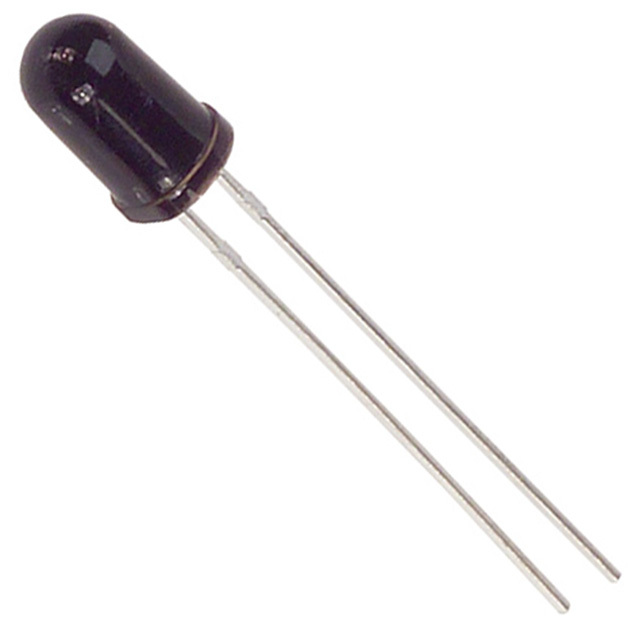
\includegraphics[width=0.2\textwidth]{phototransistor}
    \caption{Phototransistor}
    \label{fig:real_ph}
\end{figure}